\emph{\textbf{Réfraction de la lumière et indice de réfraction}}

\emph{\textbf{1. Définition - Indice de réfraction (n) ~ }}

\emph{\textbf{L'indice de réfraction} \textbf{d'un milieu}} est le
rapport entre la vitesse de la lumière dans l'air (notée c) et la
vitesse de la lumière dans le milieu considéré. Il sera noté n.

L'\textbf{indice de réfraction} d'un milieu est une grandeur sans
dimension, caractéristique d'un milieu, et décrivant le comportement de
la lumière dans celui-ci.

c étant la vitesse de la lumière dans l'air (quasi égale à la vitesse de
la lumière dans le vide), l'indice de réfraction de l'air est égal à 1.

\begin{figure}
\centering
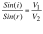
\includegraphics[width=1.804cm,height=1.413cm]{Pictures/100000010000002B00000022B156AA6818DBA2EC.png}
\caption{}
\end{figure}

Intégrons cet indice dans la loi de Snell~:

\begin{figure}
\centering
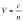
\includegraphics[width=1.399cm,height=1.268cm]{Pictures/100000010000001700000015C406BF942DA0A30B.png}
\caption{}
\end{figure}

Tenant compte de la définition de l'indice de réfraction,

nous avons que la vitesse v de la lumière dans un milieu est~:

\begin{figure}
\centering
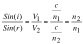
\includegraphics[width=4.445cm,height=2.328cm]{Pictures/10000001000000530000002C34DF98E92A29FA75.png}
\caption{}
\end{figure}

On a donc~:

\emph{\textbf{2. Conclusion~: La réfraction de la lumière obéit à la loi
suivante~: }}

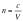
\includegraphics[width=1.646cm,height=1.505cm]{Pictures/100000010000001700000015258C94298A52913B.png}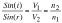
\includegraphics[width=3.903cm,height=1.434cm]{Pictures/100000010000003E0000001763CB6753C8718293.png}

\textbf{ }et

\textbf{ }

\textbf{Chaque milieu transparent est caractérisé par un indice de
réfraction qui lui est propre. }

c étant la vitesse de la lumière dans l'air (quasi égale à la vitesse de
la lumière dans le vide), l'indice de réfraction de l'air est égal à 1.

C'est la plus petite valeur pour un indice de réfraction. (le milieu est
le vide ou l'air) L'indice de réfraction du vide est quasi égal à
l'indice de réfraction de l'air.

Voici les indices de réfraction de quelques matériaux

(pour une onde lumineuse de longueur d'onde égale à 589 nm)

\hypertarget{section}{%
\section{}\label{section}}

\hypertarget{exemple-comparer-quantitativement-la-vitesse-de-la-lumiuxe8re-dans-lair-et-celle-dans-leau}{%
\section{\texorpdfstring{\emph{Exemple~}: Comparer quantitativement la
vitesse de la lumière dans l'air et celle dans
l'eau}{Exemple~: Comparer quantitativement la vitesse de la lumière dans l'air et celle dans l'eau}}\label{exemple-comparer-quantitativement-la-vitesse-de-la-lumiuxe8re-dans-lair-et-celle-dans-leau}}

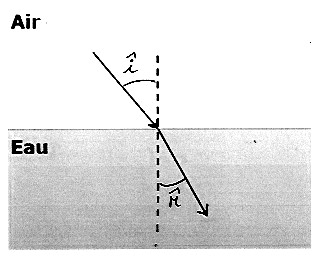
\includegraphics[width=4.852cm,height=3.941cm]{Pictures/100000010000014300000106184F9C7B3CC9C08A.png}n\textsubscript{air}
= 1

n\textsubscript{eau} = 1,33

Donc, lorsque la lumière passe de l'air à l'eau~:

\begin{figure}
\centering
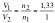
\includegraphics[width=2.926cm,height=1.221cm]{Pictures/10000001000000370000001779D0BDD76E1DB000.png}
\caption{}
\end{figure}

Donc V\textsubscript{1} = 1,33 V\textsubscript{2}

La vitesse de la lumière dans l'air est égale à 1,33 fois la vitesse de
la lumière dans l'eau.

\emph{\textbf{Application~: Décomposition de la lumière blanche à
travers un prisme}}

\begin{figure}
\centering
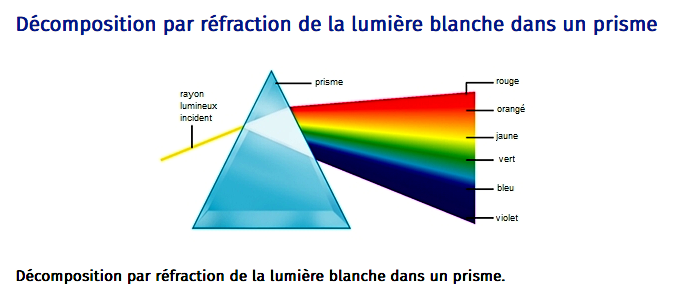
\includegraphics[width=10.968cm,height=4.81cm]{Pictures/10000001000002B20000012EAEC8536EF5F347C3.png}
\caption{}
\end{figure}

De la lumière blanche qui passe à travers un prisme est décomposée dans
toutes les couleurs de l'arc-en-ciel.

Ce phénomène est dû à la réfraction de la lumière.

Comment l'expliquer~?

\begin{figure}
\centering
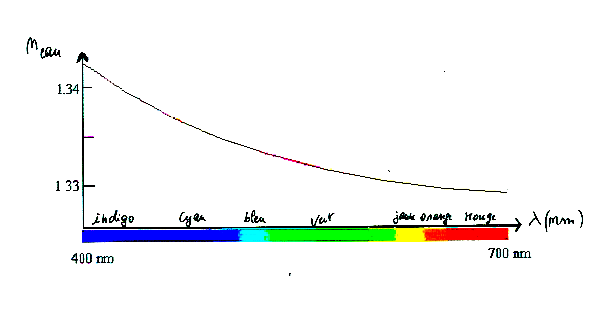
\includegraphics[width=8.366cm,height=4.369cm]{Pictures/1000000100000257000001392831DE60F0A491E3.png}
\caption{}
\end{figure}

\textbf{\textbf{L'indice de réfraction d'un milieu dépend de la longueur
d'onde de la lumière qui le traverse : l'indice est
}\emph{\textbf{légèrement plus faible}}\textbf{ pour les lumières de
longueur d'onde élevée.}}

n\textsubscript{bleu}  n\textsubscript{rouge }pour un même milieu.

Chaque couleur de la lumière blanche possède une longueur d'onde qui lui
est propre.

\textbf{\textbf{Pour certaines longueurs d'onde, la lumière sera (très
légèrement) plus lente que pour d'autres, ce qui explique que l'indice
de réfraction dépende de la longueur d'onde. }}

\textbf{}

\textbf{\textbf{Comme l'angle de réfraction est relié à l'indice de
réfraction qui est lui-même reliée à la vitesse de la lumière dans le
milieu, il est logique qu'un rayon bleu ne soit pas dévié de la même
façon qu'un rayon rouge.}}

\begin{figure}
\centering
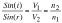
\includegraphics[width=3.903cm,height=1.434cm]{Pictures/100000010000003E0000001763CB6753C8718293.png}
\caption{}
\end{figure}

Lorsque la lumière traverse deux milieux différents, la déviation sera
plus marquée si la différence entre les indices de réfraction est
élevée. Donc, pour un même milieu n\textsubscript{1}, au plus un indice
de réfraction (n\textsubscript{2}) est grand, au plus l'angle de
réfraction sera petit. Et au plus l'angle de réfraction est petit, au
plus la déviation est grande.

Comme n\textsubscript{bleu}  n\textsubscript{rouge }(pour un même
milieu), l'angle de réfraction du bleu sera plus petit que l'angle de
réfraction du rouge et la déviation du bleu plus grande que celle du
rouge.

\emph{\textbf{La lumière bleue subira donc une plus grande déviation que
la lumière rouge lorsque de la lumière blanche traverse un prisme
(réfraction). }}

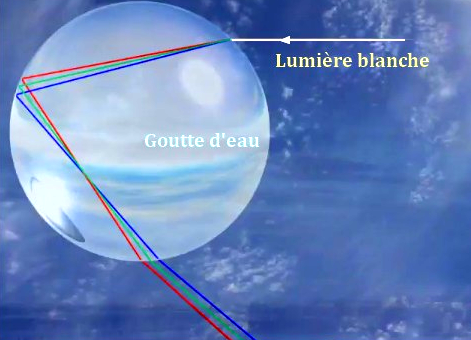
\includegraphics[width=6.669cm,height=4.81cm]{Pictures/10000001000001D700000154DEDF53D3BC2FC9C3.png}\emph{\textbf{Application~1:
l'arc-en-ciel}}

La dispersion de la lumière du Soleil par des gouttes de pluie
approximativement sphériques provoque l'arc-en-ciel. La lumière est
d'abord réfractée en pénétrant la surface de la goutte, subit ensuite
une réflexion partielle à l'arrière de cette goutte et, enfin est
réfractée à nouveau en sortant.

L'observateur verra donc la lumière blanche décomposée en toutes ses
couleurs.

\emph{\textbf{Application 2 - Interférences des couches minces (p115)}}

\begin{figure}
\centering
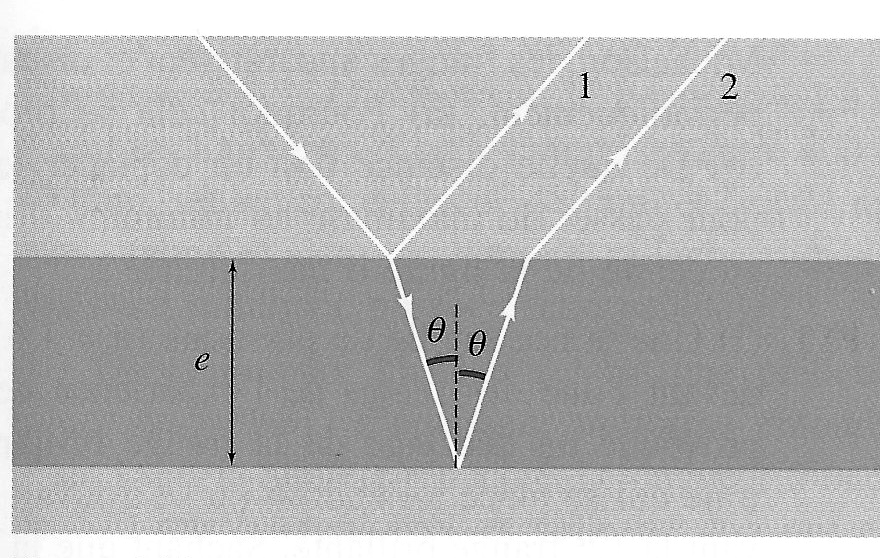
\includegraphics[width=8.266cm,height=5.228cm]{Pictures/10000000000003700000022E63EEBD01CC1425A1.png}
\caption{}
\end{figure}

Les couleurs que l'on peut observer sur des bulles de savon, des films
d'huile ou d'essence sur le sol mouillé, l'irisation de certaines plumes
de paon ou de

papillons sont dues à des phénomènes de réfraction et d'interférences.

\emph{Explication~: }

Lorsqu'une couche mince est éclairée par de la lumière blanche (une aile
de papillon par exemple, ou une tache d'huile sur la route, ou la
surface d'une DVD), une partie de la lumière est réfléchie par la
première surface et l'autre partie par la seconde surface (après avoir
subi deux réfractions). (cfr schéma)

La première onde est réfléchie par la partie supérieure de la surface.
La seconde onde subit une réfraction, une réflexion et une seconde
réfraction. Les deux ondes vont donc subir une interférence.

Comme vous le savez, chaque couleur de la lumière blanche possède une
longueur d'onde qui lui est propre.

Si l'interférence est destructive pour une certaine longueur d'onde, la
lumière aura perdu une partie de ses composantes colorées, elle n'est
plus blanche et présentera une couleur.

Comme l'épaisseur d'une couche mince varie d'un point à l'autre, les
conditions d'interférence destructives et construtives varient
également, ce qui donne toute cette variété de couleurs.

\begin{figure}
\centering
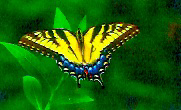
\includegraphics[width=6.398cm,height=3.881cm]{Pictures/10000001000000B50000006E88C555448F03DCAC.png}
\caption{}
\end{figure}

\emph{\textbf{Application 3 -Différence entre diffraction de la lumière
par un réseau et réfraction de la lumière. }}

\begin{figure}
\centering
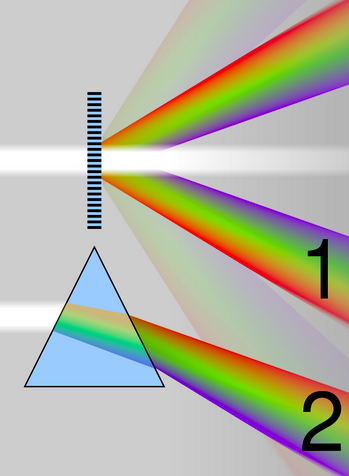
\includegraphics[width=6.015cm,height=8.193cm]{Pictures/100000010000015D000001DC81DFB5AA1CFF149A.png}
\caption{}
\end{figure}

\emph{\textbf{Figure 1~: diffraction de la lumière par un réseau}}

Rappel~: la diffraction de la lumière par un réseau et la décomposition
de la lumière blanche qui en découle est du à un phénomène
d'interférence tel que l'angle de déviation est proportionnel à la
longueur d'onde.

Comme \textsubscript{ bleu}  \textsubscript{rouge} , \textsubscript{
bleu}  \textsubscript{ rouge}

La couleur bleue subira un angle de déviation inférieur à l'angle de
déviation de la couleur rouge.

\emph{La couleur rouge subira une plus grande déviation que la couleur
bleue.}

\emph{\textbf{Figure 2~: réfraction de la lumière par un prisme}}

Rappel~: la réfraction de la lumière est due à un changement de
direction lorsqu'il y a changement de milieu. Ceci étant la conséquence
d'une variation de vitesse.

Lorsque de la lumière blanche traverse un prisme, chaque couleur subira
un angle de réfraction inversement proportionnel à son indice de
réfraction.

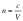
\includegraphics[width=1.646cm,height=1.505cm]{Pictures/1000000100000017000000153E95FBDB71A73A78.png}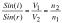
\includegraphics[width=3.903cm,height=1.434cm]{Pictures/100000010000003E000000178A699B6CC4279ED5.png}

Comme n\textsubscript{bleu}  n\textsubscript{rouge }(pour un même
milieu n\textsubscript{1} et un même angle d'incidence i),
r\textsubscript{bleu} r\textsubscript{rouge}.

\emph{La couleur bleue subira une plus grande déviation que la couleur
rouge. }

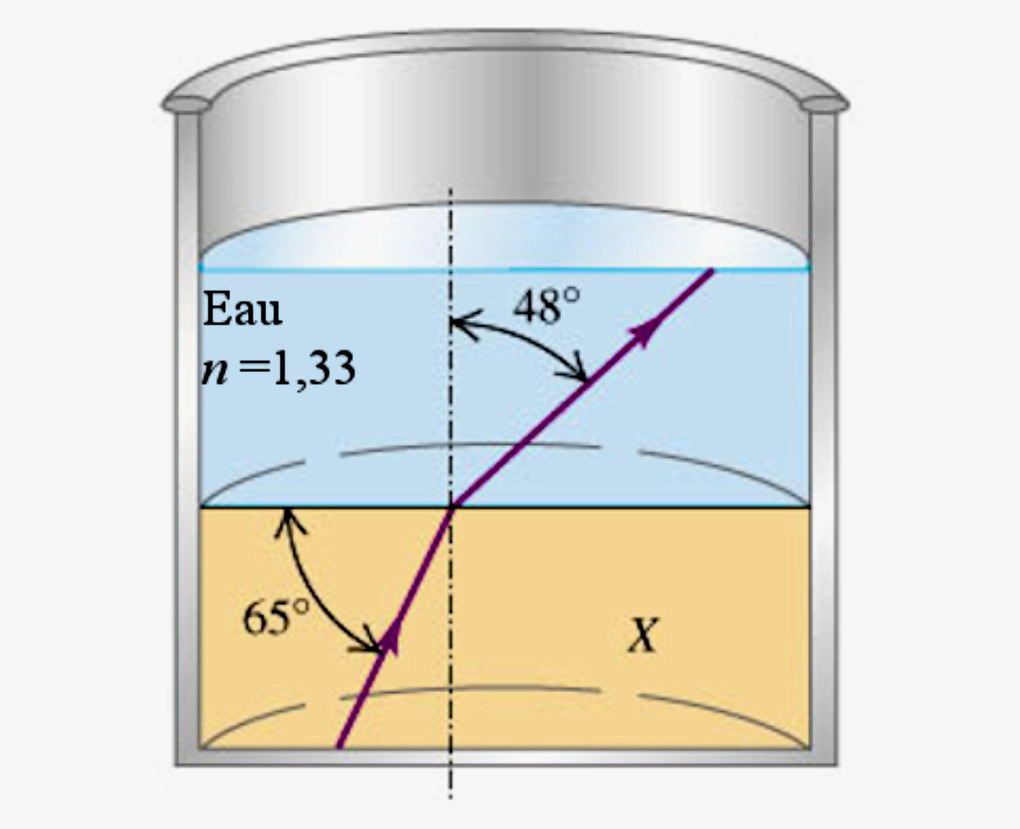
\includegraphics[width=4.711cm,height=5.338cm]{Pictures/10000001000003FC0000033DD06925E04B0F5051.png}\emph{\textbf{EXERCICE
1}}

Un rayon lumineux passe d'une substance transparente X à l'eau telle
qu'illustrée sur la figure.

a) Quel est l'indice de réfraction de la substance X? (Rép~: 2,34)

b) Quelle est la vitesse de la lumière dans la substance X~?
(Rép~:1,28.10\textsuperscript{8} m/s)

c) Quel sera l'angle limite de réflexion totale~? (Rép~: 34,5°)

\emph{\textbf{EXERCICE 2}}

\begin{figure}
\centering
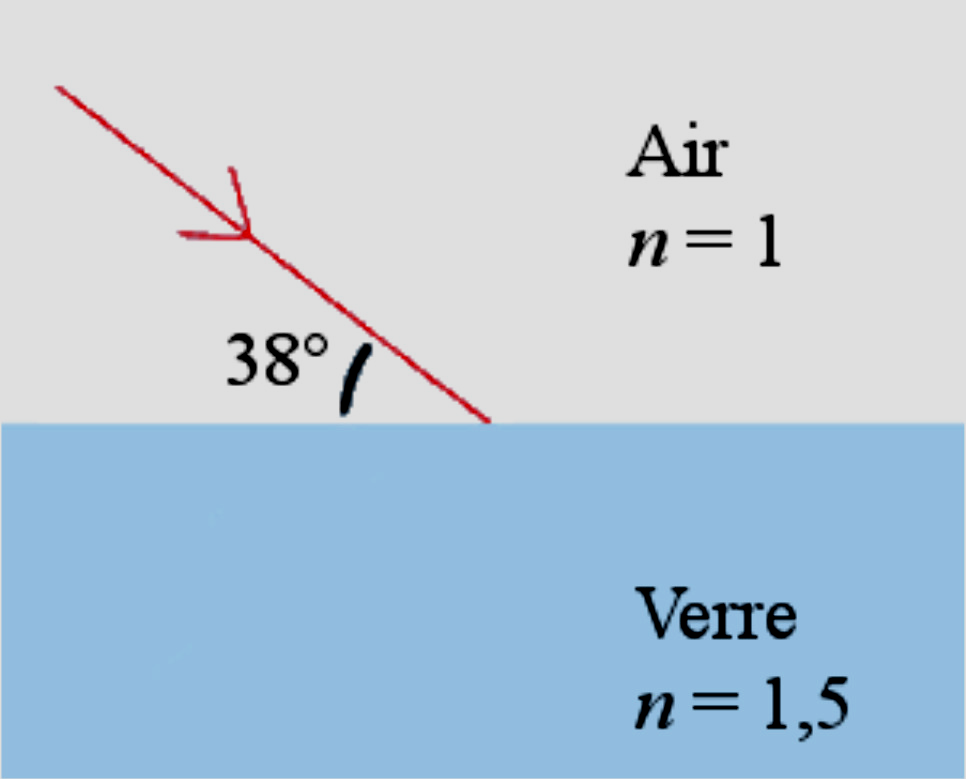
\includegraphics[width=3.475cm,height=2.801cm]{Pictures/10000001000003C60000030BB07F4672F43BCB0A.png}
\caption{}
\end{figure}

De la lumière arrive à une interface entre le verre et l'air tel
qu'illustré sur la figure.

La lumière fera-t-elle une réflexion totale ou non\textbf{ }? (Rép~:
non, dans notre situation, il n'y aura jamais de réflexion totale~:
n\textsubscript{1}n\textsubscript{2} et donc
v\textsubscript{1}v\textsubscript{2})

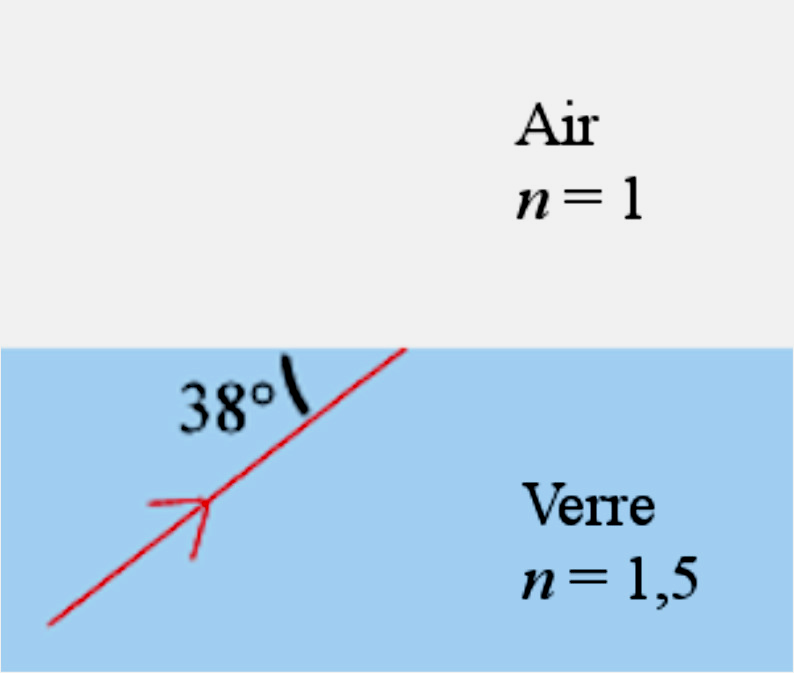
\includegraphics[width=3.246cm,height=2.75cm]{Pictures/100000010000031A000002A1271E381BD22001F0.png}\emph{\textbf{EXERCICE
3}}

De la lumière arrive à une interface entre le verre et l'air tel
qu'illustré sur la figure.

La lumière fera-t-elle une réflexion totale ou non\textbf{ }? (Rép~:
oui, ii\textsubscript{lim})

\emph{\textbf{EXERCICE 4}}

\begin{figure}
\centering
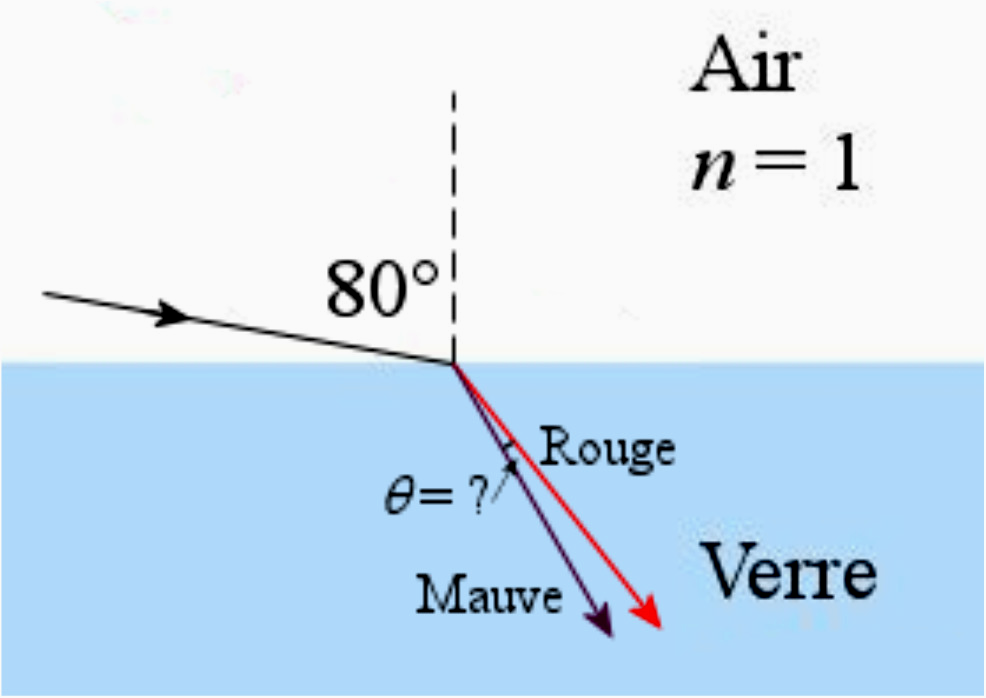
\includegraphics[width=5.944cm,height=4.209cm]{Pictures/10000001000003DA000002BA1D52E5C4A7536E3C.png}
\caption{}
\end{figure}

De la lumière blanche se propageant dans l'air arrive avec un angle
d'incidence de 80° sur la surface d'un morceau de verre.

En se réfractant dans le verre, les couleurs se séparent puisque
l'indice de réfraction n'est pas le même selon les couleurs.

L'indice passe de 1,66 pour le mauve à 1,62 pour le rouge.

Quel est l'angle entre le rayon mauve et le rayon rouge dans le
verre\textbf{ }? (Rép~: 1~,04°)

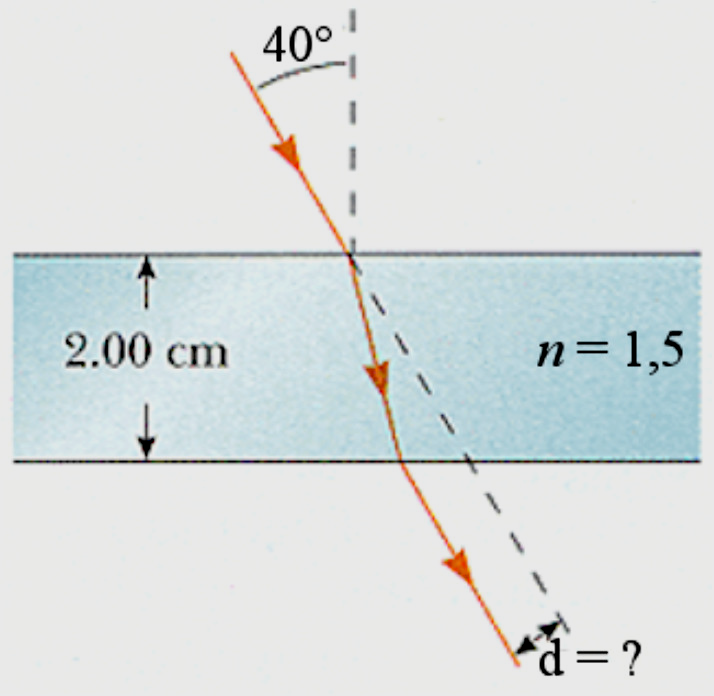
\includegraphics[width=5.597cm,height=5.456cm]{Pictures/10000001000002CA000002B85275081FCFD04057.png}\emph{\textbf{EXERCICE
5}}

Un rayon lumineux traverse une plaque de verre telle qu'illustrée sur la
figure.

Après avoir traversé le verre, le faisceau est décalé d'une distance d
par rapport à sa trajectoire initiale.

Quelle est la valeur de d? (Rép~: 5,6 mm)

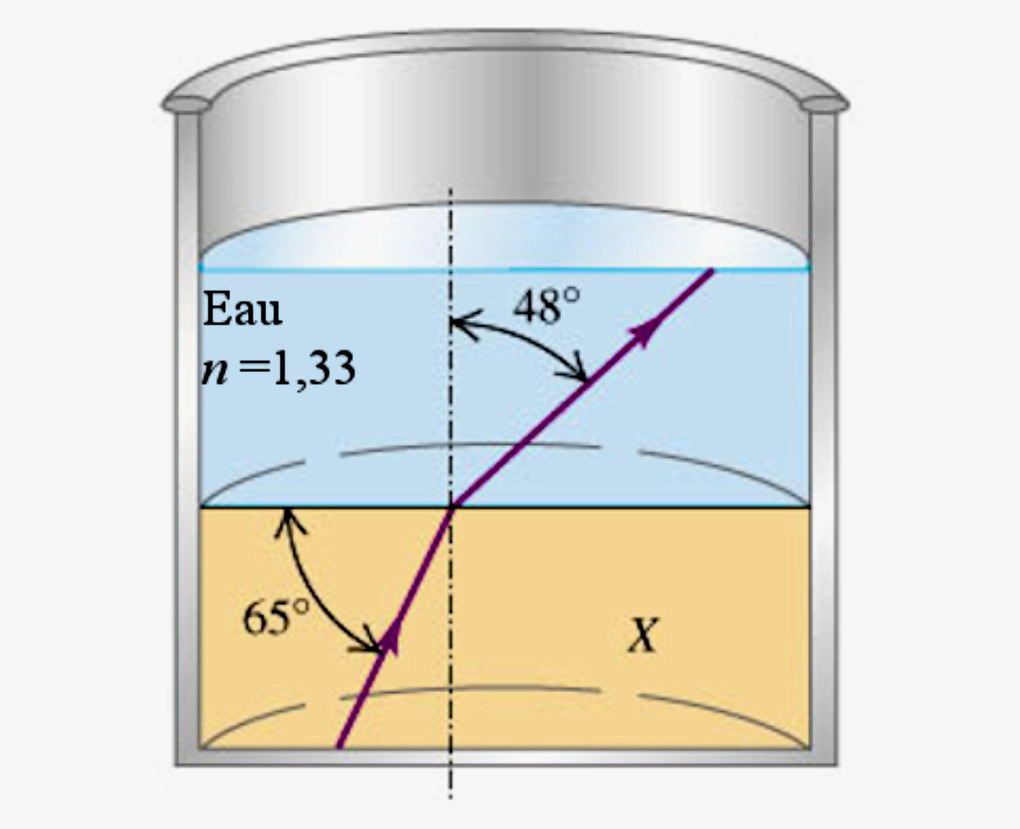
\includegraphics[width=5.927cm,height=6.713cm]{Pictures/10000001000003FC0000033DD06925E04B0F5051.png}\emph{\textbf{EXERCICE
1}}

Un rayon lumineux passe d'une substance transparente X à l'eau telle
qu'illustrée sur la figure.

a) Quel est l'indice de réfraction de la substance X?

b) Quelle est la vitesse de la lumière dans la substance X~?

c) Quel sera l'angle limite de réflexion totale~?

\begin{figure}
\centering
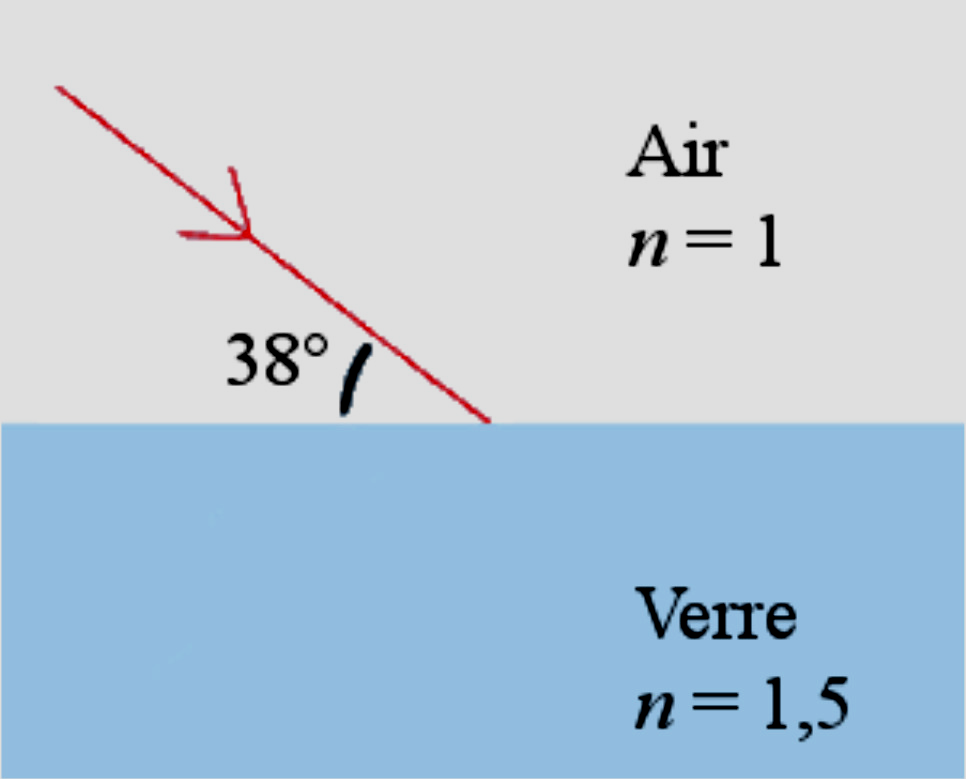
\includegraphics[width=4.745cm,height=3.826cm]{Pictures/10000001000003C60000030BB07F4672F43BCB0A.png}
\caption{}
\end{figure}

\emph{\textbf{EXERCICE 2}}

De la lumière arrive à une interface entre le verre et l'air tel
qu'illustré sur la figure.

La lumière fera-t-elle une réflexion totale ou non\textbf{ }?

\emph{\textbf{EXERCICE 3}}

\begin{figure}
\centering
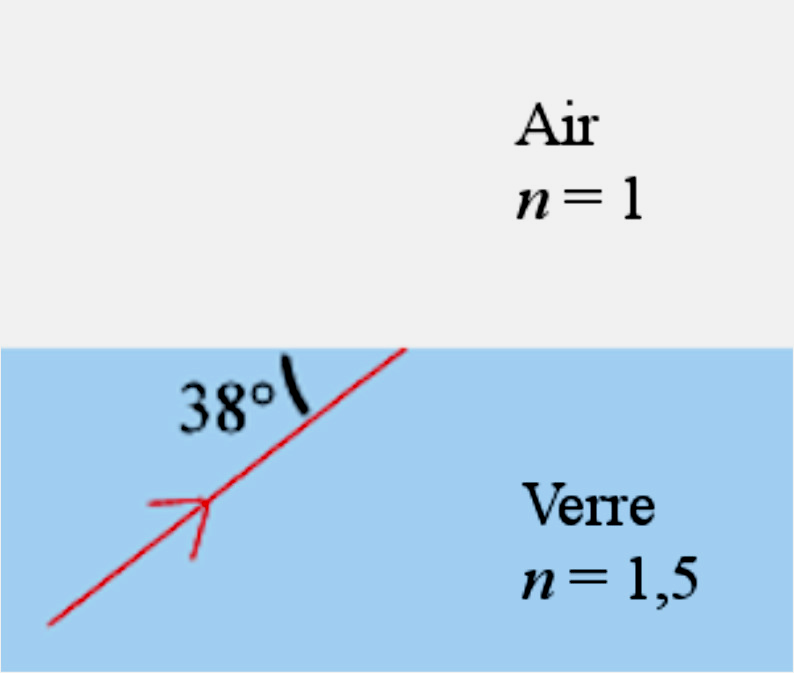
\includegraphics[width=4.175cm,height=3.538cm]{Pictures/100000010000031A000002A1271E381BD22001F0.png}
\caption{}
\end{figure}

De la lumière arrive à une interface entre le verre et l'air tel
qu'illustré sur la figure.

La lumière fera-t-elle une réflexion totale ou non\textbf{ }?

\emph{\textbf{EXERCICE 4}}

\begin{figure}
\centering
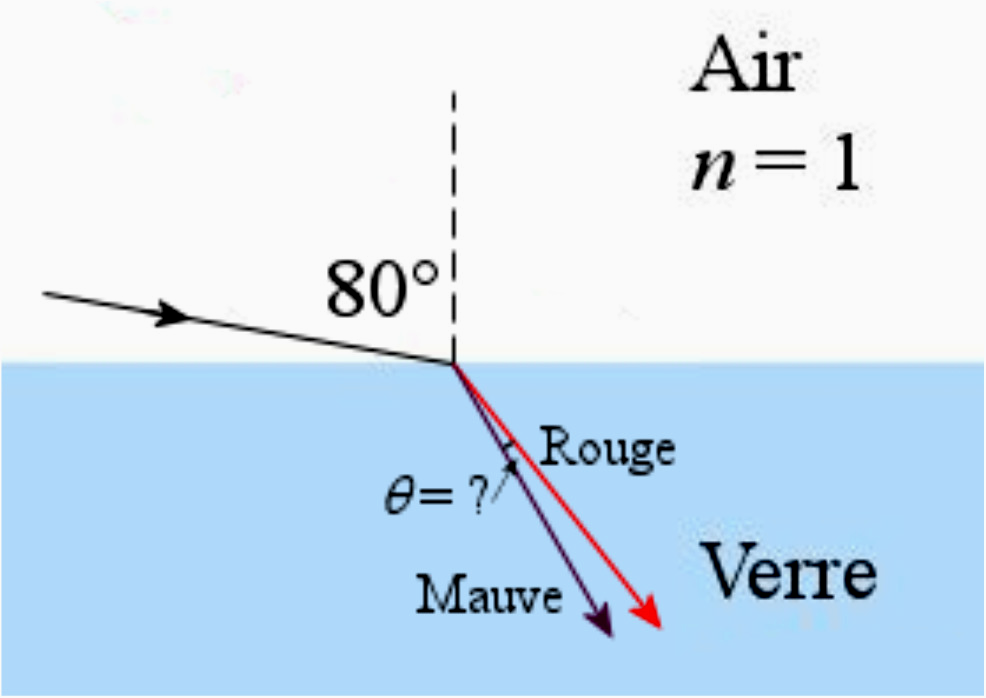
\includegraphics[width=5.944cm,height=4.209cm]{Pictures/10000001000003DA000002BA1D52E5C4A7536E3C.png}
\caption{}
\end{figure}

De la lumière blanche se propageant dans l'air arrive avec un angle
d'incidence de 80° sur la surface d'un morceau de verre.

En se réfractant dans le verre, les couleurs se séparent puisque
l'indice de réfraction n'est pas le même selon les couleurs.

L'indice passe de 1,66 pour le mauve à 1,62 pour le rouge.

Quel est l'angle entre le rayon mauve et le rayon rouge dans le
verre\textbf{ }?

\emph{\textbf{EXERCICE 5}}

\begin{figure}
\centering
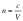
\includegraphics[width=7.257cm,height=7.073cm]{Pictures/1000000100000017000000153E95FBDB71A73A78.png}
\caption{}
\end{figure}

Un rayon lumineux traverse une plaque de verre telle qu'illustrée sur la
figure.

Après avoir traversé le verre, le faisceau est décalé d'une distance d
par rapport à sa trajectoire initiale.

Quelle est la valeur de d?

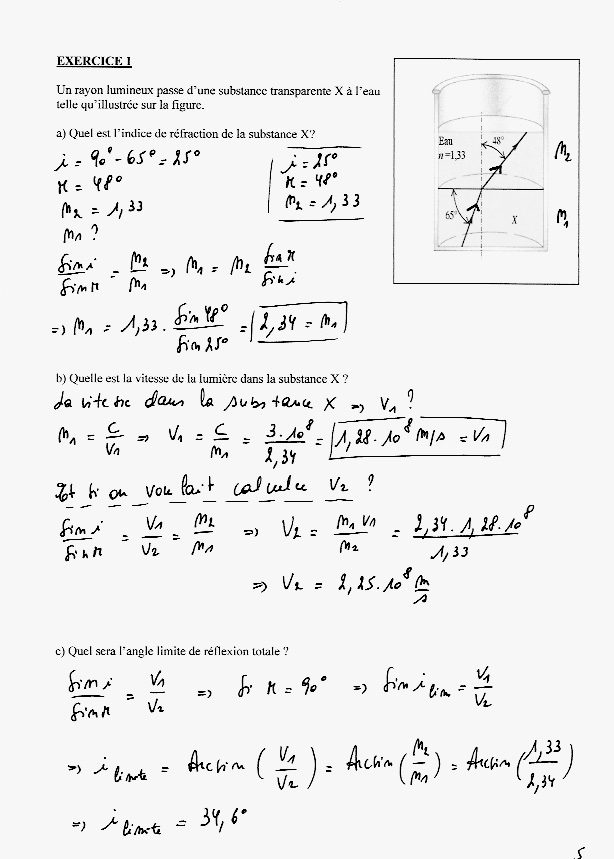
\includegraphics[width=17.503cm,height=24.477cm]{Pictures/10000001000002660000035BCA62AD70226081EC.png}

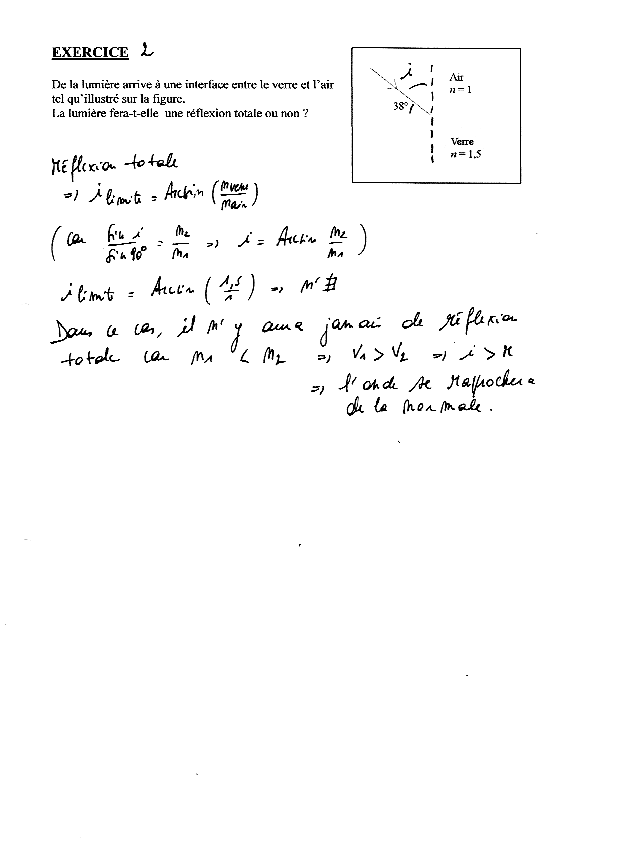
\includegraphics[width=17.503cm,height=24.231cm]{Pictures/100000010000026F0000035EE9BF0781E67AA675.png}

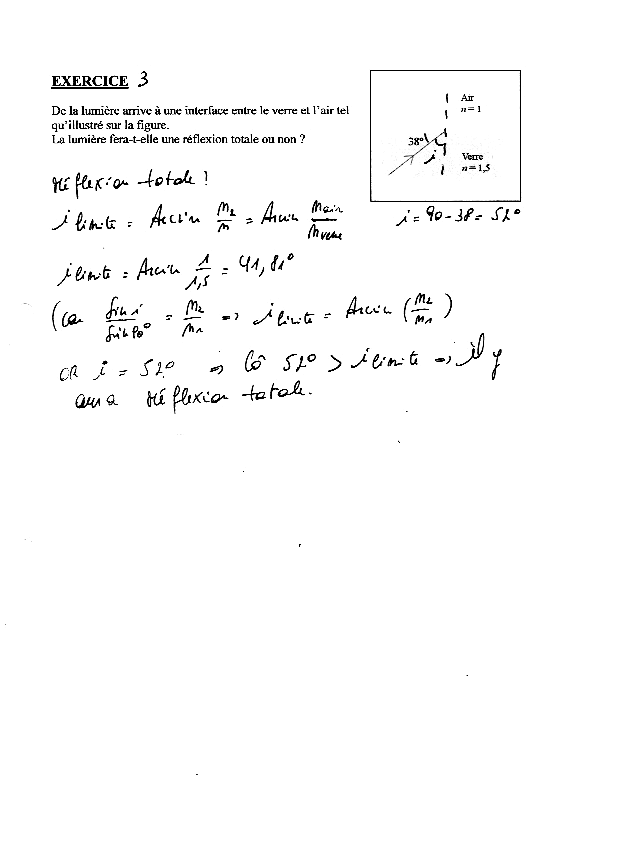
\includegraphics[width=17.503cm,height=24.231cm]{Pictures/100000010000026F0000035E9FDA6B0D4D8F454A.png}

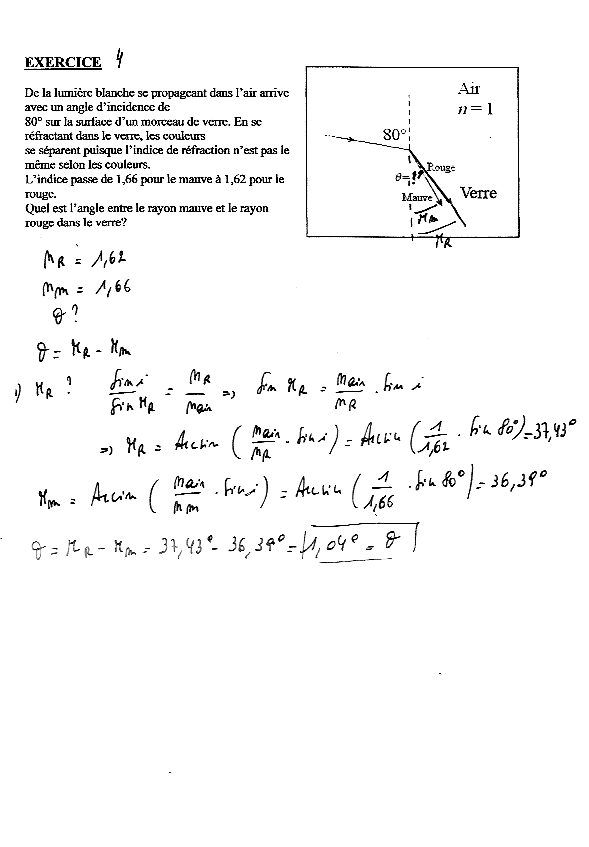
\includegraphics[width=17.503cm,height=25.174cm]{Pictures/100000010000024D0000034F56B8138A5D6394A6.png}

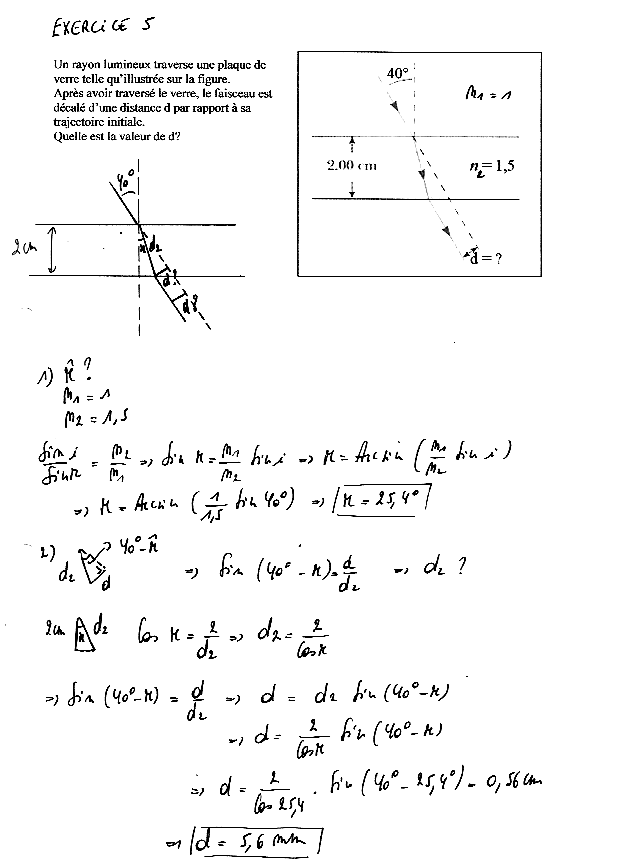
\includegraphics[width=17.503cm,height=24.231cm]{Pictures/100000010000026F0000035E2F0BA8745765B6B1.png}
